\documentclass{CCEE_UFBA_Class}

%%%%%%%%%%%%%%%%%%%%%%%%%%%%%%%%%%%%%%%%
%	Arquivo criado pelo CCEE utilizando
%   como base a classe AbnTeX2.
%   Autores: André Tahim e Cristiane Paim
%	Universidade Federal da Bahia
%	Escola Politécnica
%   Deptº de Eng. Elétrica e de Computação
%	07/01/2021
%%%%%%%%%%%%%%%%%%%%%%%%%%%%%%%%%%%%%%%%
% ---
% Informações de dados para CAPA e FOLHA DE ROSTO
% -------------------------------------------------------------------------------
\titulo{Título do Projeto de TCC}
\autor{Ricardo Augusto de Araújo Machado}
\orientador{Orientador: Prof. Dr. André Pires Nóbrega Tahim}
%\coorientador{Coorientador: Prof. Dr. Y} % Comente se nao existir.
\local{Salvador-Ba -- Brasil}
\data{2025}
\tipotrabalho{Relatório técnico}
% -------------------------------------------------------------------------------


\begin{document}
	
% Seleciona o idioma do documento (conforme pacotes do babel)
%\selectlanguage{english}
\selectlanguage{brazil}

% Retira espaço extra obsoleto entre as frases.
\frenchspacing 

% ----------------------------------------------------------
% ELEMENTOS PRÉ-TEXTUAIS
% ----------------------------------------------------------
% \pretextual

% ---
% Capa
% ---
\imprimircapa

% ---
% Folha de rosto
% (o * indica que haverá a ficha bibliográfica)
% ---
%\imprimirfolhaderosto*
% ---
\cleardoublepage
% ---
% inserir o sumario
% ---
\pdfbookmark[0]{\contentsname}{toc}
\tableofcontents*
\cleardoublepage
% ---


% ----------------------------------------------------------
% ELEMENTOS TEXTUAIS
% ----------------------------------------------------------
\textual
	
%%%%%%%%%%%%%%
%	CAPÍTULOS
%%%%%%%%%%%%%%
\chapter{Introdução}
Atualmente, o setor de transportes corresponde a 30\% e 31\% da matriz energética dos Estados
Unidos e dos países da União Europeia, respectivamente \cite{eia_transportation_energy} e
\cite{eurostat_transport_energy}. Tendo em vista que é necessário reduzir a emissão de gases do
efeito estufa significativamente nos próximos anos, a eletrificação do setor automobilístico é
uma medida importante para atingir o objetivo supracitado. Ao mesmo tempo, a ausência de uma
infraestrutura de carregamento robusta e a falta de autonomia são os maiores gargalos para a
adoção em massa de veículos elétricos.

O desenvolvimento de uma infraestrutura de carregamento deve ser planejado para não
sobrecarregar a rede elétrica e respeitar tanto a norma da Aneel Nº 414/201, que limita o fator
de potência para valores a partir de 0,92 quanto as normas relativas à distorção harmônica
máxima permitida como, por exemplo, a norma europeia IEC 61000-3-2 e a norma chinesa GB
17625.1-2022 . Dessa forma, um carregador de veículo elétrico obrigatoriamente precisa
apresentar um estágio ativo de correção do fator de potência. Ademais, a fim de garantir uma
maior autonomia para essa categoria de veículos, é necessário que os carregadores forneçam uma
potência suficientemente alta.

Os carregadores de veículos elétricos podem ser \emph{on-board} ou \emph{off-board}. No
primeiro caso, o veículo é conectado diretamente à rede elétrica e o circuito de potência
interno do automóvel realiza a retificação da tensão de entrada CA para CC. No último caso, as
estações de carregamento realizam o processo de retificação e conversão de energia e fornecem
para o veículo uma tensão de alimentação CC.

Considerando os desafios existentes para a utilização em massa de veículos elétricos, este
trabalho visa projetar e simular um carregador \emph{on-board} trifásico bidirecional completo,
incluindo tanto o estágio do PFC quanto o estágio do conversor CC-CC.

\chapter{Definição do Problema de Estudo}

A estrutura básica de um veículo elétrico é exibida na Figura
\ref{fig:estrutura-veiculo-eletrico}. O bloco conversor CA-CC no diagrama representa todo o
carregador \textit{onboard} do veículo elétrico, incluindo tanto o retificador PFC quanto o
conversor CC-CC isolado. O sistema de carregamento pode ser unidireccional ou bidirecional. No
primeiro caso, o sistema apenas converte a energia da rede elétrica para o veículo, enquanto no
segundo caso, o veículo pode fornecer energia de volta para a rede elétrica, o que é conhecido
como \textit{Vehicle-to-Grid} (V2G). O banco de baterias do veículo é composto por células de
lítio e ultracapacitores, que são ulizados para armazenar a energia elétrica fornecida pelo
carregador. O inversor é responsável por converter a tensão CC da bateria em uma tensão CA, que
aciona o motor do sistema de tração do veículo. Como ilustrado no diagrama, o inversor
geralmente é bidirecional, o que permite o uso de frenagem regenerativa.

Os carregadores de veículos elétricos são divididos em carregadores \textit{onboard}(OBC) e
\textit{offboard}. Os carregadores \textit{onboard} são instalados dentro do veículo e são
projetados para serem leves e compactos, devido a restrições de espaço e peso. A potência de
saída desses carregadores está na faixa de 0 a 7 kW para sistemas monofásicos e de 0 a 22 kW
para sistemas trifásicos \cite{Yuan:2021}. Já os carregadores \textit{offboard} também são
chamados de carregadores nível 3 e já fornecem uma tensão CC direta para o veículo, ignorando o
OBC conforme ilustrado na Figura \ref{fig:diagrama-bypass-offboard}. A potência de saída desses
carregadores é significativamente maior, variando de 120 kW a 240 kW, segundo
\cite{texas:2020}.

\begin{figure}[htb]
    \centering
    \caption{Estrutura básica de um veículo elétrico.}
    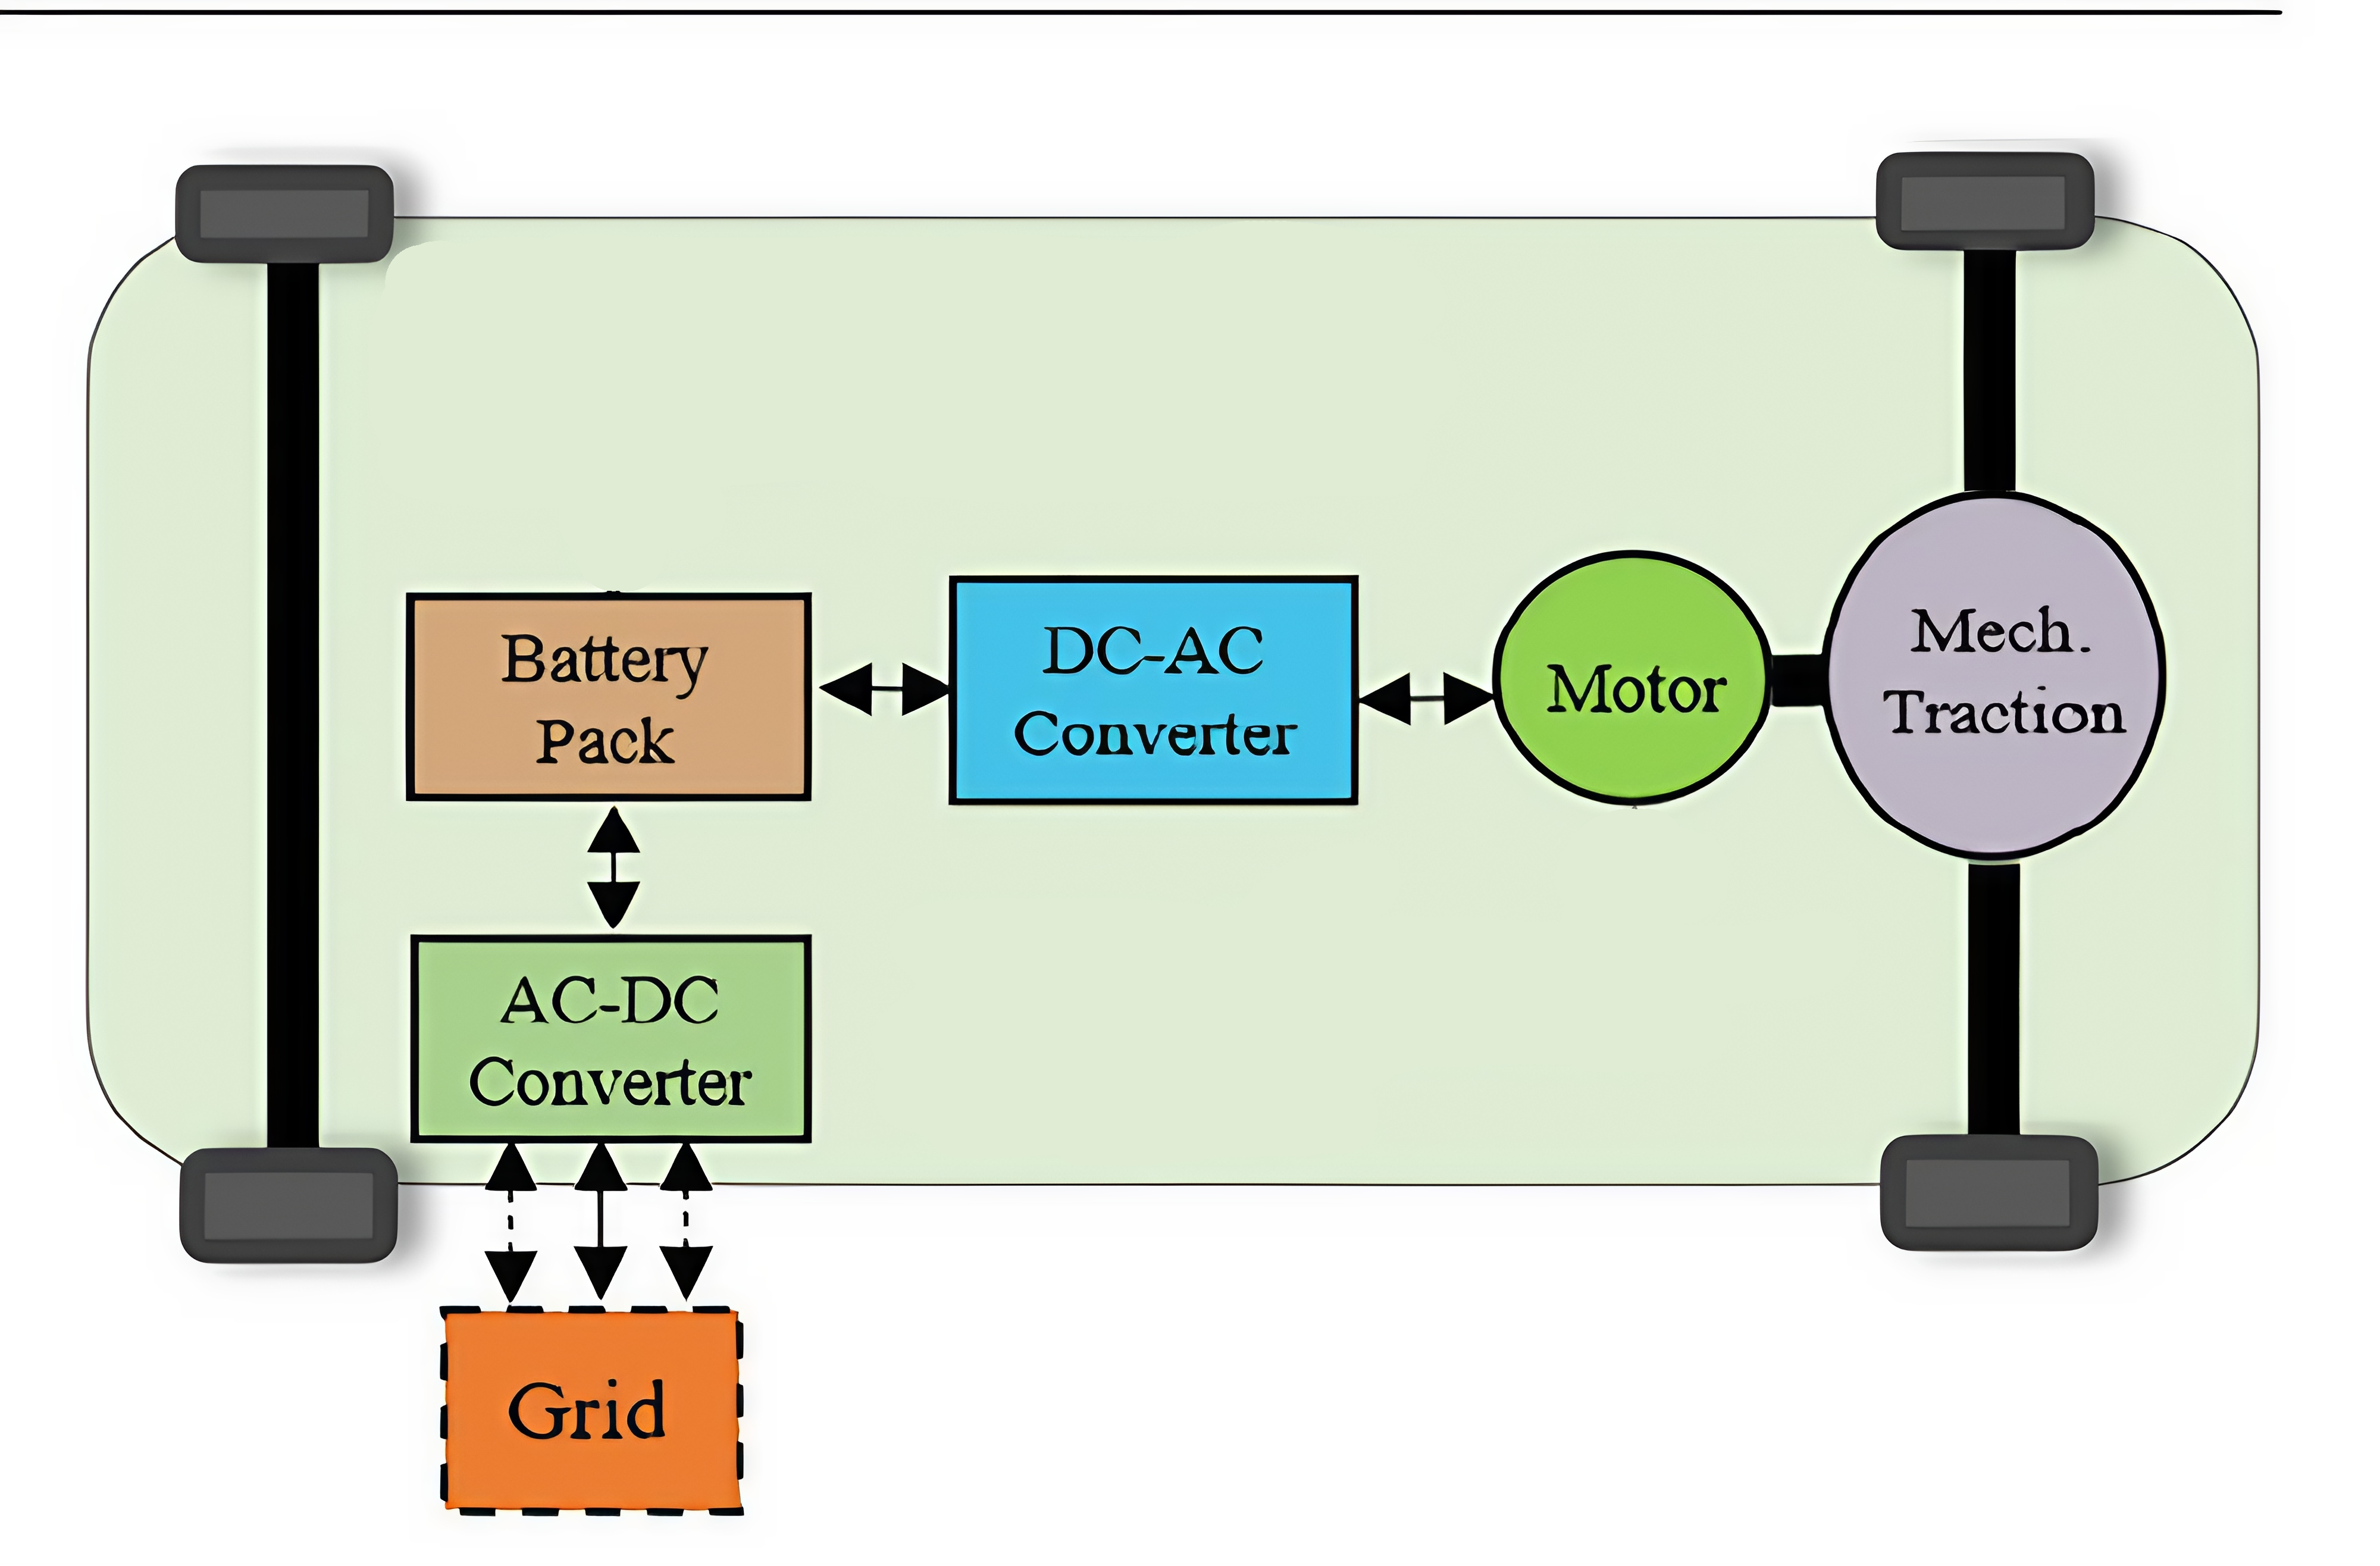
\includegraphics[width=0.8\textwidth]{Figuras/diagrama_veiculo_eletrico_edit.png}
    \legend{Fonte: Adaptado de \cite{Kumar:2021}.}
    \label{fig:estrutura-veiculo-eletrico}
\end{figure}

\begin{figure}[htb]
    \centering
    \caption{Sistema de carregamento \textit{offboard}. Há uma conexão direta entre o
        carregador e a bateria do veículo.}
    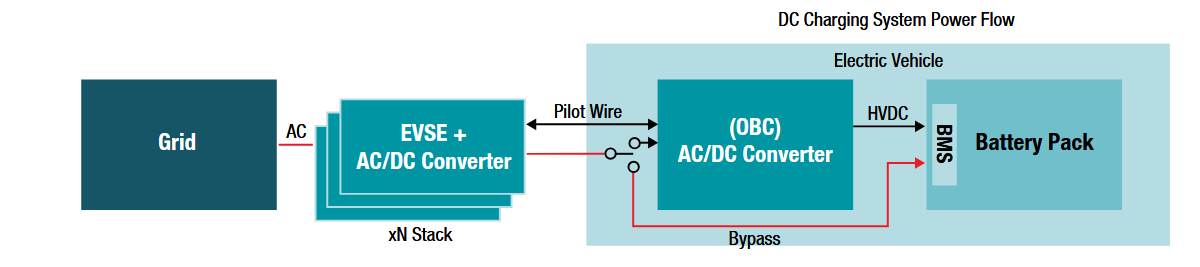
\includegraphics[width=0.8\textwidth]{Figuras/diagrama_bypass.png}
    \legend{Fonte: \cite{texas:2020}.}
    \label{fig:diagrama-bypass-offboard}

\end{figure}

A crescente demanda por veículos elétricos é impulsionada pela necessidade de reduzir emissões
de gases do efeito estufa e a dependência de combustíveis fósseis. De acordo com
\cite{anfavea2024descarbonizacao}, num cenário de transição gradual, é previsto que 65\% da
frota de veículos no Brasil seja elétrica até 2035. No entanto, a adoção em massa de veículos
elétricos enfrenta gargalos significativos, especialmente no que diz respeito à falta de
infraestrutura de carregamento e à baixa autonomia dos veículos elétricos \cite{Karneddi:2021}.

Ademais, os carregadores de veículos elétricos devem ser projetados para não afetar de forma
significativa a rede de distribuição elétrica, principalmente em relação ao fator de potência e
a distorção harmônica total. Nesse quesito, a normas técnicas IEC 61000-3 e GB/T 14549,
vigentes na União Europeia e na China, respectivamente, estabelecem limites de distorção
harmônica total e fator de potência para equipamentos conectados à rede elétrica. No Brasil, a
seção VIII da resolução 1000/2021 da ANEEL estabelece o fator de potência mínimo de 0,92 para
consumidores do grupo A, com cobrança de multa para excesso de energia reativa
\cite{aneel_ren1000_2021}.

Considerando os desafios encontrados para a crescente demanda em veículos elétricos, o seguinte
trabalho propõe o projeto de um carregador \textit{onboard} que seja adequado à realidade do
sistema de distribuição brasileiro. Dessa forma, escolhe-se trabalhar com um sistema de
carregamento trifásico que funcione com a rede de distribuição elétrica das grandes capitais
brasileiras, caracrterizada por uma tensão de fase de 127 \(V_{\mathrm{rms}}\) e uma frequência
de 60 Hz. O carregador será composto por um retificador PFC trifásico, que garante o fator de
potência próximo a unidade, e um conversor CC-CC isolado, que pode ser um \textit{Phase-Shifted
    Full Bridge}, um \textit{Dual Active Bridge}(DAB) ou um conversor ressonante. No trabalho será
realizado a comparação entre o \textit{Phase-Shifted Full Bridge} e o DAB com o objetivo de
verificar qual topologia apresenta melhor desempenho.

\section{Objetivo Geral}
O objetivo geral do trabalho é projetar um carregador de veículo elétrico \textit{onboard}
trifásico, composto por um retificador PFC e um conversor CC-CC isolado.
\section{Objetivos Específicos}
\begin{itemize}
    \item Revisão bibliográfica sobre as diferentes topologias utilizadas nos carregadores de veículos
          elétricos;
    \item Projeto do circuito retificador PFC trifásico;
    \item Sintonia do controlador do retificador PFC trifásico;
    \item Revisão bibliográfica sobre conversores CC-CC isolados;
    \item Projeto do conversor CC-CC \textit{Phase-Shifted Full Bridge};
    \item Projeto do conversor CC-CC \textit{Dual Active Bridge}(DAB);
    \item Comparação entre o \textit{Phase-Shifted Full Bridge} e o DAB.
    \item Integração dos estágios do carregador.
\end{itemize}

\chapter{Revisão Bibliográfica}
Neste capítulo reúne-se as fontes de pesquisa que vão fornecer o embasamento teórico para o seu 
trabalho. É na revisão da literatura onde deve-se apresentar os trabalhos relacionados ao tema 
ou cuja solução pode ser aplicada ao problema de estudo. A revisão bibliográfica não é um 
conjunto de trecho de obras, mas uma apresentação pessoal e crítica dos trabalhos anteriormente 
realizados. Recomenda-se realizar uma revisão bibliográfica com os seguintes passos:
\begin{enumerate}
	\item Escolha boas referências – Encontre autores e obras especializadas no tema do seu trabalho de TCC.
	\item Analise as referências – Verifique se as referências têm relação direta com o recorte do seu problema.
	\item Crie um padrão – Esse padrão pode ser cronológico, ou pode ser classificada por tipo de solução. Ex. Um problema de controle pode ser abordado por técnicas de controle lineares e não-lineares. Assim, a sua revisão pode ser dividida por ordem cronológica em que os trabalhos foram apresentados ou classificados por soluções de controle lineares e não-lineares. 
	\item Faça uma análise crítica das referências – Leia as obras, analise-as e faça anotações. Sintetize o conteúdo de cada obra e reflita sobre cada teoria/solução apresentada de modo a destacar a sua visão crítica. Dessa forma, a sua revisão não será um mero enxerto de passagens da literatura.
\end{enumerate}

Em relação ao retificador PFC trifásico, tanto \cite{3phPlecs} quanto \cite{WANG2013/03} 
realizam o controle desse conversor por meio da transformada de Park.  Nessa metodologia, há 
duas malhas de controle, uma externa, referente a tensão de saída do retificador e uma interna,
 que controla as componentes de eixo direto e em quadratura da corrente de entrada.

\chapter{Solução e Avaliação da Proposta}
\section{Solução Proposta}
Esta seção é destinada a explicação de como você resolverá o problema, ou como você pretende
realizar o projeto. Neste estágio é preciso estar claro o que você irá fazer, mas flexível o
suficiente para adaptar a solução a adversidades encontradas durante a realização do projeto. A
escrita da proposta da solução não o previne do insucesso, mas permite que você identifique
diversos problemas com antecedência. Note que a metodologia descrita aqui é dependente do tipo
de projeto do seu TCC. Você deve discutir com seu orientador sobre isso.

Conforme a Figura \ref{fig:controlepfc3ph}, o controle do PFC trifásico

\begin{figure}
    \centering
    \caption{Esquema de controle do PFC trifásico.}
    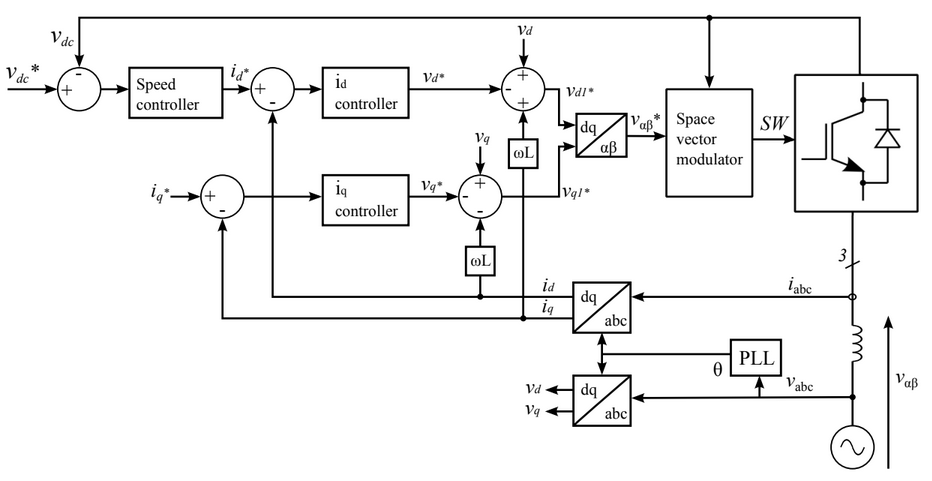
\includegraphics[width=0.8\textwidth]{./Figuras/controlepfc3ph.png}
    \legend{Fonte: \cite{3phPlecs}.}
    \label{fig:controlepfc3ph}
\end{figure}

\section{Avaliação da Solução}
Esta seção deve conter uma explicação de como será feita a avaliação da solução uma vez que ela
estiver concluída. O método de avaliação é dependente do projeto e o seu orientador pode
guiá-lo para a forma de avaliação mais adequada.

\chapter{Resultados Preliminares}
Este capítulo é facultativo! Caso o seu trabalho tenha alcançado algum resultado preliminar, ele deve ser incluído aqui. Deve-se destacar que para qualquer simulação (ou experimento) o aparato utilizado e os procedimentos seguidos para obtenção dos resultados devem ser detalhadamente apresentados. \emph{A descrição da sua simulação (ou experimento) deve conter informações suficientes para que o leitor possa repliclá-lo}. Frequentemente figuras bem elaborados conseguem condensar e dar uma ideia esclarecedora de como os resultados foram obtidos, tais como: fotos de bancada, diagrama de blocos, esquemáticos, fluxogramas, etc. É importante para qualquer engenheiro/pesquisador adquirir a habilidae de descrever/ilustrar a essência de como os resultados foram obtidos.

\chapter{Cronograma e Recursos}
\section{Cronograma}

Cada etapa do projeto deve produzir algum resultado. Assim, o processo de planejamento deve
produzir um cronograma de metas, indicando quando cada objetivo deve ser concluído. Tal
cronograma deve conter objetivos mensuráveis, em que cada etapa produz um resultado específico.
Por exemplo, se você pretende utilizar três semanas em leitura de obras, o resultado deve ser
uma seção de revisão bibliográfica para o seu trabalho de final de graduação e não apenas a
leitura das obras. Esta etapa deve conter uma tabela de tarefas a serem realizadas dentro de um
período de tempo determinado para alcançar cada objetivo específico.

\section{Recursos}

Apresente uma estimativa do que será necessário para realizar o projeto. Indique os recursos de
hardware, software ou orçamento necessário para realizar o projeto. Esta etapa é importante
para destacar a viabilidade do projeto. Dessa forma, qualquer ferramenta necessária para
execução do projeto e sua disponibilidade deve estar incluída nesta seção.

\begin{table}[h]
    \centering
    \caption{Lista de recursos para o trabalho de conclusão de curso.}
    \label{tab:recursos}
    \begin{tabular}{|l|l|}
        \hline
        Recurso          & Categoria      \\ \hline
        Computador       & Recurso Físico \\ \hline
        Osciloscópio     & Recurso Físico \\ \hline
        Fonte CC         & Recurso Físico \\ \hline
        Carga Eletrônica & Recurso Físico \\ \hline
        MATLAB           & Software       \\ \hline
        PSIM             & Software       \\ \hline
    \end{tabular}
\end{table}

% ----------------------------------------------------------
% ELEMENTOS PÓS-TEXTUAIS
% ----------------------------------------------------------
\postextual

\bibliographystyle{./Auxiliares/abntex2-alf}
\bibliography{./Auxiliares/ref-TCC}

%% ---
% Inicia os apêndices
% ---
\begin{apendicesenv}

% Imprime uma página indicando o início dos apêndices
%\partapendices

% ----------------------------------------------------------
\chapter{Informações e Dicas \LaTeX}
% ----------------------------------------------------------

Este apêndice contém algumas dicas para escrita de um documento técnico em \LaTeX no formato ABNT.

\section{Inserindo Citações}

\textbf{Latex:}
\begin{verbatim}
Imagine que isso é um texto que necessita de uma citação
\cite{Kasper:2014}. Talvez mais uma informação seja necessária
\cite{Liu:2011}.
\end{verbatim}

\textbf{Resultado:}\\
Imagine que isso é um texto que necessita de uma citação \cite{Kasper:2014}. Talvez mais uma informação seja necessária \cite{Liu:2011}.

\section{Inserindo Equações}

\textbf{Latex:}
\begin{verbatim}
\begin{equation}
\cos (2\theta) = \cos^2 \theta - \sin^2 \theta
\end{equation}.
\end{verbatim}

\textbf{Resultado:}\\
\begin{equation}
\cos (2\theta) = \cos^2 \theta - \sin^2 \theta
\end{equation}.
\newpage
\section{Citando Equações}

Para citar uma equação é necessário dar um nome pra equação (um label), no exemplo abaixo a equação foi rotulada de \textit{eq:cos2theta}:

\textbf{Latex:}
\begin{verbatim}
\begin{equation}
\label{eq:cos2theta}
\cos (2\theta) = \cos^2 \theta - \sin^2 \theta
\end{equation}.

Para citá-la apenas utilize o comando eqref. 

Ex. Substituindo \eqref{eq:cos2theta} em...  
\end{verbatim}



\textbf{Resultado:}\\
\begin{equation}
\label{eq:cos2theta}
\cos (2\theta) = \cos^2 \theta - \sin^2 \theta
\end{equation}.

Para citá-la apenas utilize o comando eqref. 

Ex. Substituindo \eqref{eq:cos2theta} em... 

\newpage
\section{Inserindo Figuras}

\subsection{Inserindo uma Figura}
\textbf{Latex:}
\begin{verbatim}
\begin{figure}[htb]
\caption{\label{fig:farol-da-barra}Farol da Barra}
\begin{center}
\includegraphics[width=0.7\linewidth]{./Figuras/farol-da-barra.jpg}
\end{center}
\legend{Fonte: os autores}
\end{figure}
\end{verbatim}

\textbf{Resultado:}
\begin{figure}[htb]
	\caption{\label{fig:farol-da-barra}Farol da Barra}
	\begin{center}
		\includegraphics[width=0.7\linewidth]{./Figuras/farol-da-barra.jpg}
	\end{center}
	\legend{Fonte: os autores}
\end{figure}

Eu agora irei citar a Figura \ref{fig:farol-da-barra}

\newpage
\subsection{Inserindo Figuras Lado a Lado}

\textbf{Latex:}
\begin{verbatim}
\begin{figure}[!htb]
\label{teste}
\centering
\begin{minipage}{0.45\textwidth}
\centering
\caption{Imagem 1 da minipage} \label{fig:poli1}
\includegraphics[width=1\linewidth]{./Figuras/poli1}
\legend{Fonte: Produzido pelos autores}
\end{minipage}
\hfill
\begin{minipage}{0.45\textwidth}
\centering
\caption{Imagem 2 da minipage} \label{fig:poli2}
\includegraphics[width=1\linewidth]{./Figuras/poli1}
\legend{Fonte: o autor}
\end{minipage}
\end{figure}
\end{verbatim}


\textbf{Resultado:}
\begin{figure}[!htb]
	\label{teste}
	\centering
	\begin{minipage}{0.45\textwidth}
		\centering
		\caption{Imagem 1 da minipage} \label{fig:poli1}
		\includegraphics[width=1\linewidth]{./Figuras/poli1}
		\legend{Fonte: Produzido pelos autores}
	\end{minipage}
	\hfill
	\begin{minipage}{0.45\textwidth}
		\centering
		\caption{Imagem 2 da minipage} \label{fig:poli2}
		\includegraphics[width=1\linewidth]{./Figuras/poli1}
		\legend{Fonte: o autor}
	\end{minipage}
\end{figure}

\end{apendicesenv}

\end{document}